\section{Introducción}

El presente trabajo practico consiste en tomar la imagen patrón \textit{lenna.bmp} (\ref{fig:lenna}) y aplicar diferentes filtros a las imágenes para  obtener diferentes resultados, luego se utiliza un banco de filtro para mostrar las aplicaciones que tiene sobre el filtrado de las imágenes.

Se mostraran los resultados obtenidos de los diferentes filtro. La idea del filtrado de imagen consiste que a cada sub-matriz de pixeles de la imagen de \textit{NxN} se la multiplique por una matriz de \textit{NxN} obteniendo así una matriz con combinación de cada pixel. Matemáticamente se puede expresar como

\begin{equation}
	\begin{bmatrix}
		p_1 & \ldots & p_N\\
		\vdots & \ddots & \vdots\\
		p_N & \ldots & p_N
	\end{bmatrix} \times 
	\begin{bmatrix}
		a_1 & \ldots & a_N\\
		\vdots & \ddots & \vdots\\
		a_N & \ldots & a_N
	\end{bmatrix}=	\begin{bmatrix}
		b_1 & \ldots & b_N\\
		\vdots & \ddots & \vdots\\
		b_N & \ldots & b_N
	\end{bmatrix}
\end{equation}
\begin{equation}
	\textbf{P}\times \textbf{A} = \textbf{B}
\end{equation}


en donde cada $b_i$ sera una combinación lineal entre el pixel $p_i$ y los coeficientes $a_i$. La matriz \textbf{A} que es generada por los coeficientes $a_i$, termina siendo el filtro que se aplica, mientras que la matriz \textbf{P} seria la matriz de los pixeles. En este trabajo usaremos diferentes tipos de filtros y mostraremos la imagen resultante al aplicar el filtro, ademas calcularemos el histograma de cada uno de los filtros. Para terminar, se usara un banco de filtro para mostrar aplicaciones que se pueden tener sobre los diferentes imágenes.

\begin{figure}[H]
	\centering
	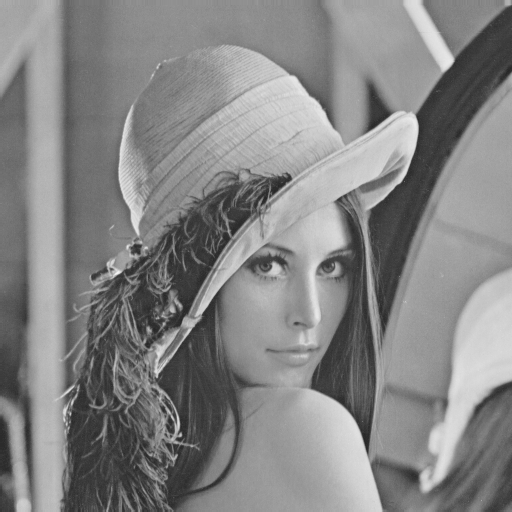
\includegraphics[scale=0.5]{imagenes/original.png}
	\caption{Imagen resultante en escala de grises\label{fig:lenna}.}
\end{figure}

\section{Desarrollo}

\subsection{Filtros}

Para simplificar las cuentas tomaremos filtros de \textit{3x3}, usaremos matrices \textbf{A} filtro conocidos, como entre ellos \textit{Laplace} que transforman a la imagen en diferentes aspectos. Explicaremos con mas detalle cada filtro.

\subsubsection{Blur}

El filtro \textit{Blur} consiste en un suavizado a la imagen, toma los pixeles y multiplica cada pixel por valores $a_i$. Generalmente los coeficientes $a_i$ son generados por una normal multivarible de dos dimensiones por lo que la matriz del filtro es simétrica. Debido a esto ultimo, tambien es conocido este filtro como \textit{Gaussian Blur}.
Para la imagen resultante, se usa la siguiente matriz \textbf{A}:

\begin{equation}
\textbf{A}=\begin{bmatrix}
0.0625 &0.125 &0.0625\\
0.125 &0.25 &0.125\\
0.0625 &0.125 &0.0625
\end{bmatrix}
\end{equation}

al aplicar el filtro se puede obtener la imagen (\ref{fig:blur}) donde se observa que la imagen es mas borrosa que la original. Se puede entender mirando la diferencia entre los histogramas de ambas imágenes, el filtro blur contiene la energia de la imagen mas distribuida entre todo el rango de los pixeles generando un histograma mas continuo, al tener la energía mas distribuida genera que la intensidad de cada pixel (altura del histograma) sea mas baja provocando un efecto borroso.

\begin{figure}[H]
	\centering
	\subfigure[Imagen original]{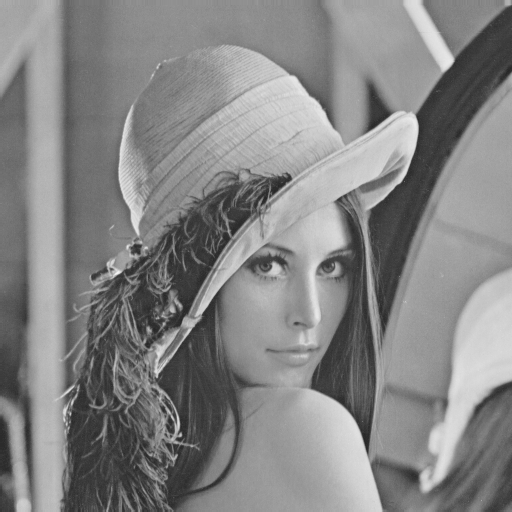
\includegraphics[scale=0.4]{imagenes/original.png}}
		\subfigure[Imagen filtrada con el filtro \textit{Blur}]{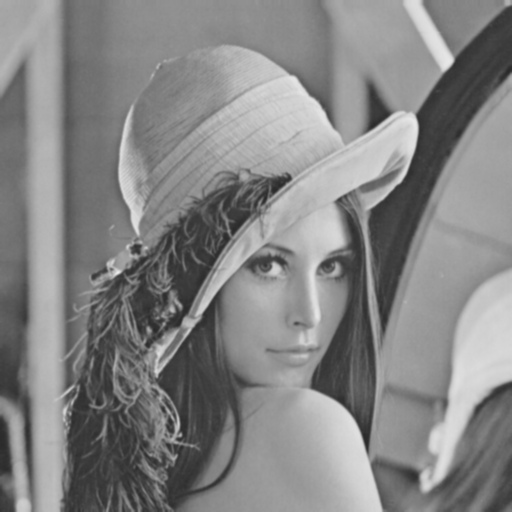
\includegraphics[scale=0.4]{imagenes/blur.png}}
	\caption{Comparación de las imágenes\label{fig:blur}.}
\end{figure}	

\begin{figure}[H]
	\centering
	\subfigure[Histograma de la imagen original]{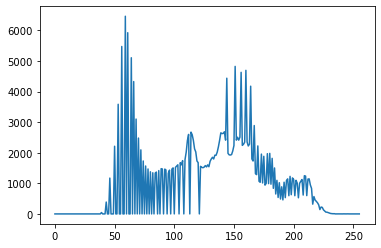
\includegraphics[scale=0.5]{imagenes/histOriginal.png}}
		\subfigure[Histograma de la imagen filtrada por \textit{Blur}]{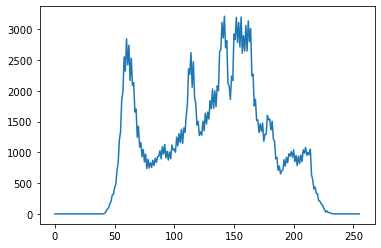
\includegraphics[scale=0.5]{imagenes/histBlur.png}}
	\caption{Comparación de los histogramas de las imágenes.}
\end{figure}	

\subsection{Sobel}

El filtro de \textit{Sobel} se usa principalmente para la detección de bordes. Como vimos en los trabajos prácticos, esto va a depender mucho del recorrido entonces puedo definir diferentes forma la matriz de \textit{Sobel} para obtener los mismo resultados. Las matrices de \textit{Sobel} mas comunes son \textit{bottom}, \textit{top} , \textit{left} y \textit{rigth}. La matriz de \textit{Sobel} proviene del gradiente de la función intensidad de una imagen.

\subsubsection{Bottom Sobel}

El \textit{Bottom Sobel} consiste sobre los pixeles que se le aplica el gradiente de la función de intensidad. La matriz \textbf{A} para el \textit{Bottom Sobel} viene dada por

\begin{equation}
\textbf{A}=\begin{bmatrix}
-1 &-2 &-1\\
0 &0 &0\\
1 &2 &1
\end{bmatrix}
\end{equation}

en donde se observa que para algunos pixeles se le aplica el gradiente de la función intensidad mientras que en otros se anula la intensidad. Se considera \textit{Bottom Sobel} sobre donde se encuentra en gradiente de la función intensidad.

\subsubsection{Top Sobel}

Al igual que \textit{Bottom Sobel} consiste en donde se encuentra el gradiente obteniendo la matriz \textbf{A}

\begin{equation}
\textbf{A}=\begin{bmatrix}
1 &2 &1\\
0 &0 &0\\
1 &2 &1
\end{bmatrix}
\end{equation}

se puede observar que es la matriz \textbf{A} de \textit{Bottom Sobel} pero multiplicada por un -1. Se debe a que se esta aplicando el mismo metodo solo que el gradiente se aplica a diferentes pixeles.

\subsubsection{Left Sobel}

El \textit{Left Sobel} sigue aplicando el gradiente de la función de intensidad, solo que el gradiente se encuentra a la izquierda de la matriz \textbf{A} como se observa

\begin{equation}
\textbf{A}=\begin{bmatrix}
1 &0 &-1\\
2 &0 &-2\\
1 &0 &-1
\end{bmatrix}
\end{equation}

\subsubsection{Right Sobel}

Por ultimo, esta el método \textit{Right Sobel} que consiste en aplicar el gradiente a la derecha, se puede obtener la matriz \textbf{A} multiplicando a la matriz \textbf{A} de \textit{Left Sobel} por -1 obteniendo

\begin{equation}
\textbf{A}=\begin{bmatrix}
-1 &0 &1\\
-2 &0 &2\\
-1 &0 &1
\end{bmatrix}
\end{equation}


\subsubsection{Imágenes sobre el método Sobel}

	En la figura (\ref{fig:sobel}), se puede observar las imágenes resultantes con un filtro de \textit{Sobel}.  Al mirar la diferencia entre las distintas matrices \textbf{A} sobre todos los metodos \textit{Sobel} se puede observar que hay contornos que se muestran mejor que otros que va dependiendo en donde se aplico el gradiente. En este método no se calculo el histograma porque obtendríamos una delta sobre los pixeles de menor valor debido a que la imagen es negra salvo por el contorno.

\begin{figure}[H]
	\centering
	\subfigure[Imagen original]{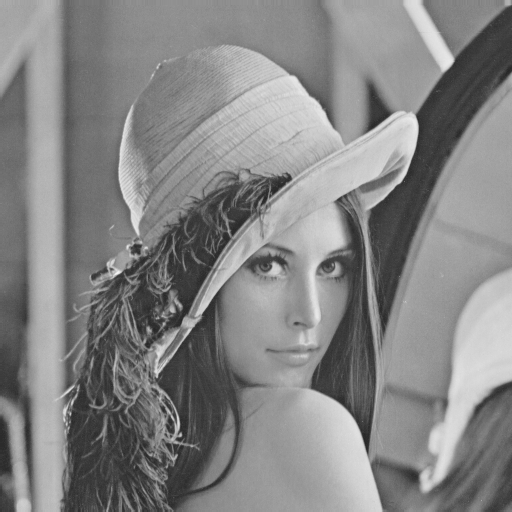
\includegraphics[scale=0.25]{imagenes/original.png}}
	\subfigure[Imagen filtrada por \textit{Bottom Sobel}]{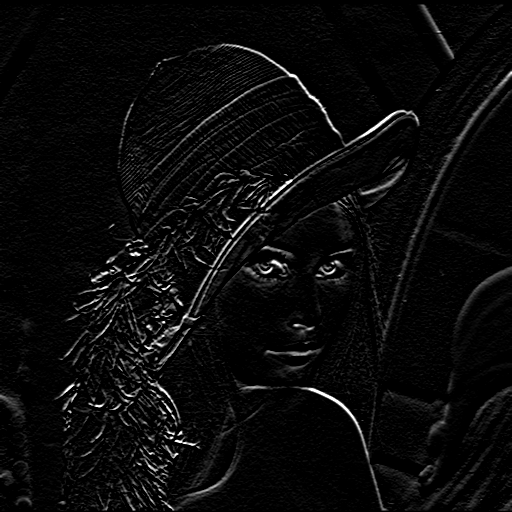
\includegraphics[scale=0.25]{imagenes/bottomSobel.png}}
	\subfigure[Imagen filtrada por \textit{Top Sobel}]{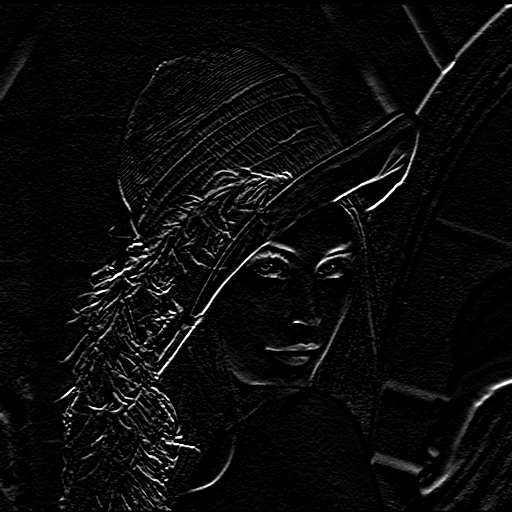
\includegraphics[scale=0.25]{imagenes/topSobel.png}}
	\subfigure[Imagen filtrada por \textit{Left Sobel}]{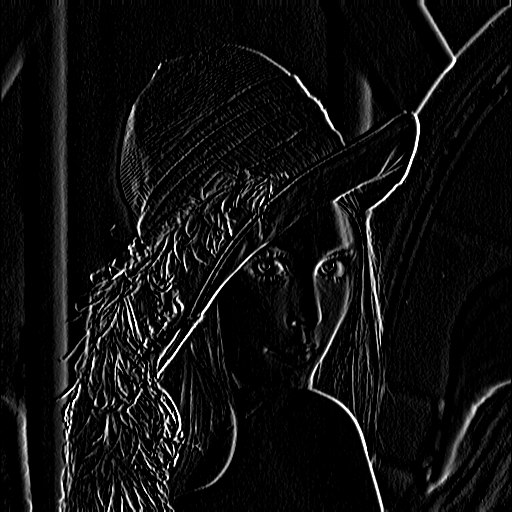
\includegraphics[scale=0.25]{imagenes/leftSobel.png}}
	\subfigure[Imagen filtrada por \textit{Right Sobel}]{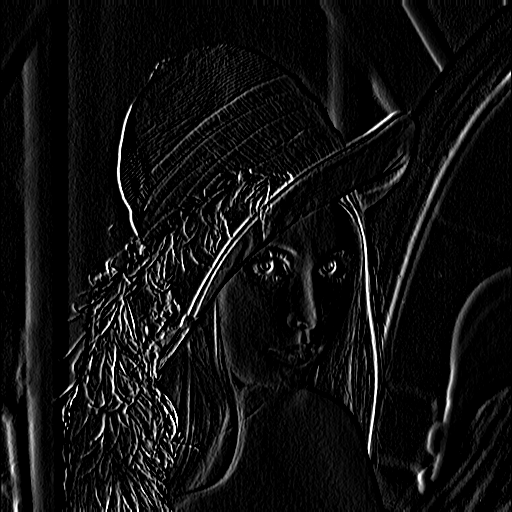
\includegraphics[scale=0.25]{imagenes/rightSobel.png}}
	\caption{Comparación de las imágenes resultante\label{fig:sobel}.}
\end{figure}	

\subsection{Emboss}

El filtro \textit{Emboos} es parecido al filtro \textit{Sobel} pero la diferencia que dala ilusión de profundidad por hacer énfasis sobre los diferentes pixeles en una dirección. El filtro reemplaza cada pixel de la imagen original por un realce o una sombra sobre el pixel dependiendo de la imagen original. La matriz \textbf{A} se obtiene a partir de

\begin{equation}
\textbf{A}=\begin{bmatrix}
-2 &-1 &0\\
-1 &1 &1\\
0 &1 &2
\end{bmatrix}.
\end{equation}

La imagen resultante termina siendo los contornos de la imagen original. A diferencia de la tecnica \textit{Sobel} se tiene que los contornos se encuentra en un fondo blanco por lo que el histograma daria una delta en los pixeles mas altos por lo que no se calculo al igual que en el \textit{Sobel}. La imagen resultante termina siendo 

\begin{figure}[H]
	\centering
	\subfigure[Imagen original]{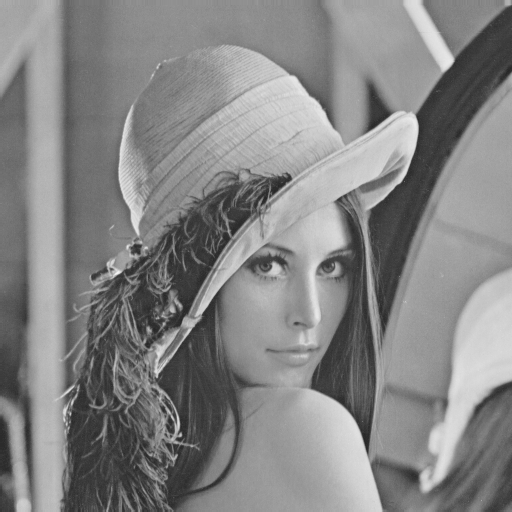
\includegraphics[scale=0.4]{imagenes/original.png}}
		\subfigure[Imagen filtrada con el filtro \textit{Emboss}]{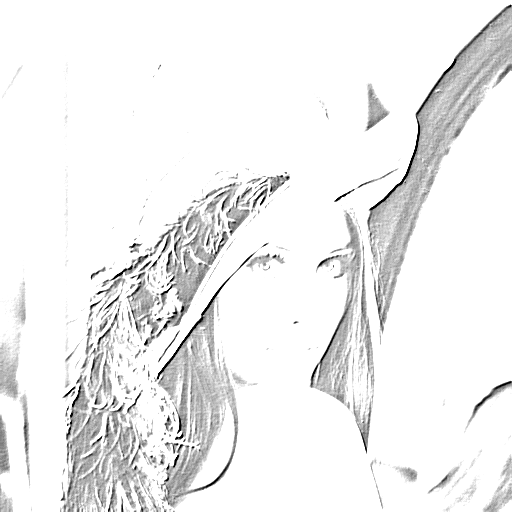
\includegraphics[scale=0.4]{imagenes/emboss.png}}
	\caption{Comparación de las imágenes\label{fig:emboss}.}
\end{figure}	

\subsection{Outline}

Un método para realce de la diferencia de los pixeles se termina usando el filtro \textit{Outline}. Consiste en ver los pixeles vecinos con lo mas cercanos con la misma intensidad. Obtiene una imagen de apariencia negra porque toma diferencia entre pixeles (valor demasiado chico salvo en un contorno) por lo que no se calcula el histograma. La matriz de \textbf{A} termina siendo

\begin{equation}
\textbf{A}=\begin{bmatrix}
-1 &-1 &-1\\
-1 &8 &-1\\
-1 &-1 &-1
\end{bmatrix}.
\end{equation}

donde se observa que se toma la diferencia entre los pixeles vecinos. El valor de 8 en el pixel del medio viene dado que estoy tomando los 8 pixeles vecinos a ese pixel. Entonces el resultado obtenido es

\begin{figure}[H]
	\centering
	\subfigure[Imagen original]{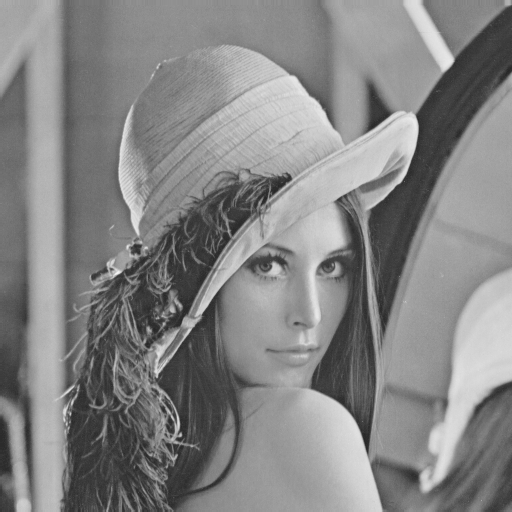
\includegraphics[scale=0.4]{imagenes/original.png}}
		\subfigure[Imagen filtrada con el filtro \textit{Outline}]{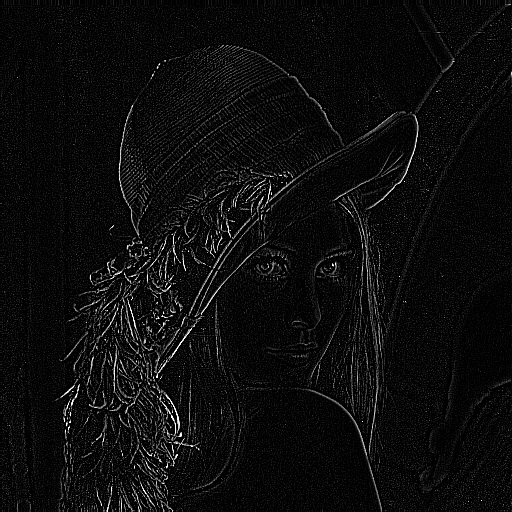
\includegraphics[scale=0.4]{imagenes/outline.png}}
	\caption{Comparación de las imágenes.}
\end{figure}	

\subsection{Laplace}

El metodo de \textit{Laplace} es parecido al metodo de \textit{Outline}, vuelve a tomar la diferencia entre los pixeles vecinos pero con la diferencia que toma los pixeles que se encuentran arriba, abajo, derecha e izquierda del pixel, poniendo la diagonales con un valor de intensidad de 0. Representando eso en una matriz se obtendria la matriz \textbf{A} como


\begin{equation}
\textbf{A}=\begin{bmatrix}
0 &-1 &0\\
-1 &4 &-1\\
0 &-1 &0
\end{bmatrix}.
\end{equation}

donde el valor de 4 corresponde a los 4 vecinos que estoy tomando sobre el pixel central. Entonces, la imagen obtenida sera parecida a la imagen conseguida con \textit{Outline} pero con menos detalles por la cantidad de direcciones que se tomaron, obteniendo 


\begin{figure}[H]
	\centering
	\subfigure[Imagen original]{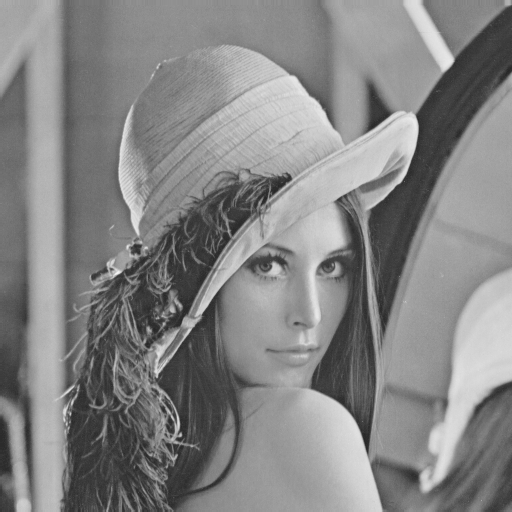
\includegraphics[scale=0.4]{imagenes/original.png}}
		\subfigure[Imagen filtrada con el filtro \textit{Laplace}]{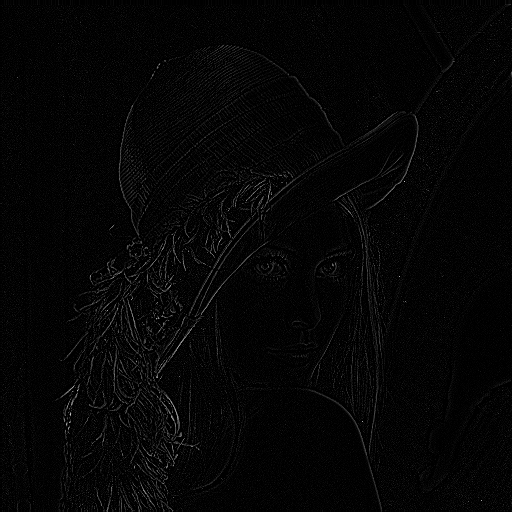
\includegraphics[scale=0.4]{imagenes/laplace.png}}
	\caption{Comparación de las imágenes.}
\end{figure}	

\subsection{Sharpen}

 Al igual que \textit{Laplace} el metodo de \textit{Sharpen} toma la diferencia entre los valores adyacente y no los diagonales, la diferencia entre \textit{Laplace} viene dada por la intensidad que se toma del pixel central, se tuma una cantidad mayor dando una imagen mas viva que en \textit{Laplace}, esto se podria enteder a que estas tomando un poco mas de energia en el pixel central por las diferencias que estas tomando. La matriz \textbf{A} se calcula como
 
 \begin{equation}
\textbf{A}=\begin{bmatrix}
0 &-1 &0\\
-1 &5 &-1\\
0 &-1 &0
\end{bmatrix}.
\end{equation}

este metodo se hizo para demostrar que cambiando el valor del pixel central del filtro se puede tener otra imagen muy diferente. En la figura (\ref{fig:sharpen}), se observa la diferencia entre la imagen original y la imagen generada por \textit{Sharpen} notandose que esta ultima es mas viva a comparacion de la original, esto se debe que el histograma de sharpen tiene una distribución diferente que la original esto se observa en la figura (\ref{fig:sharpenhist})

\begin{figure}[H]
	\centering
	\subfigure[Imagen original]{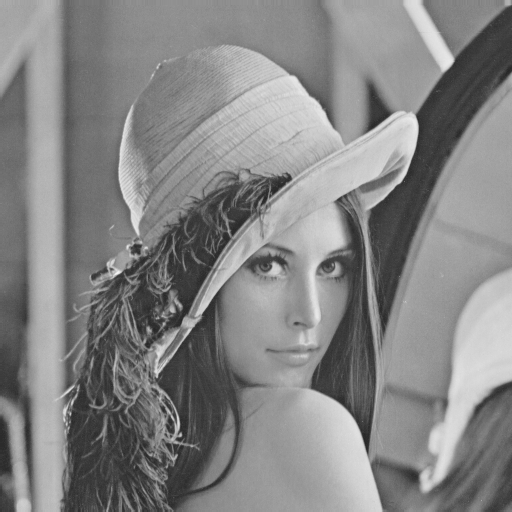
\includegraphics[scale=0.4]{imagenes/original.png}}
		\subfigure[Imagen filtrada con el filtro \textit{Sharpen}]{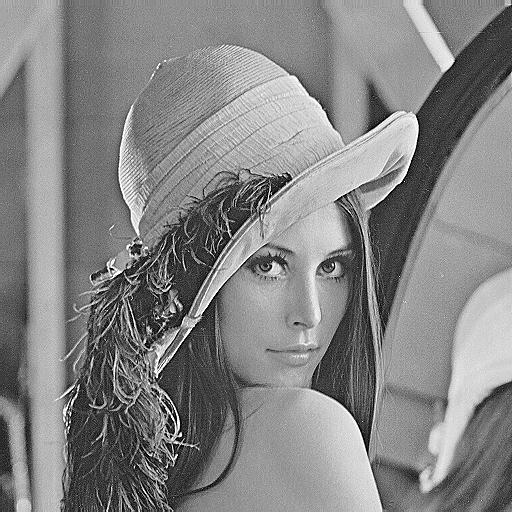
\includegraphics[scale=0.4]{imagenes/sharpen.png}}
	\caption{Comparación de las imágenes\label{fig:sharpen}.}
\end{figure}	

\begin{figure}[H]
	\centering
	\subfigure[Histograma de la imagen original]{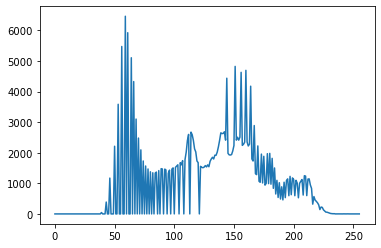
\includegraphics[scale=0.5]{imagenes/histOriginal.png}}
		\subfigure[Histograma de la imagen filtrada por \textit{Sharpen}]{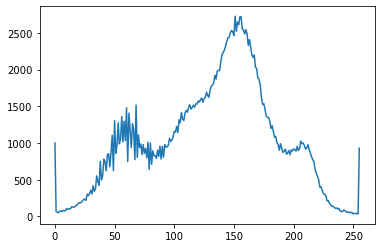
\includegraphics[scale=0.5]{imagenes/histsharpen.png}}
	\caption{Comparación de los histogramas de las imágenes\label{fig:sharpenhist}.}
\end{figure}	

\subsection{Kernel}

Por ultimo, el metodo de \textit{Kernel} se usa para disfocar la imagen, tomando la suma de los pixeles vecinos pero dividiendo la intensidad por un numero mayor a 1 asi se reduce la intensidad de cada pixel. En forma de matriz \textbf{A} se expresa como 

 \begin{equation}
\textbf{A}=\frac{1}{25}\begin{bmatrix}
1 &1 &1\\
1 &1 &1\\
1 &1 &1
\end{bmatrix}.
\end{equation}

mostrando que cada pixel es dividido por un numero mayor a 1, logrando la apariencia de disfocado. La imagen resultante comparada con la imagen original se puede observar en la figura (\ref{fig:kernel}). El disfocado se observa en el histograma como la reducción de la intensidad del mismo. Los resultados se observan a continuación


\begin{figure}[H]
	\centering
	\subfigure[Imagen original]{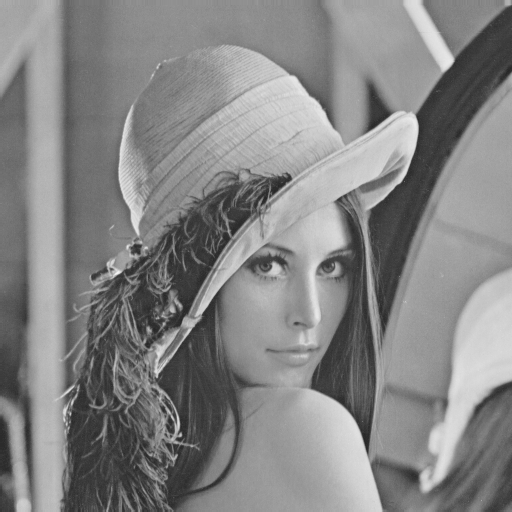
\includegraphics[scale=0.4]{imagenes/original.png}}
		\subfigure[Imagen filtrada con el filtro \textit{Kernel}]{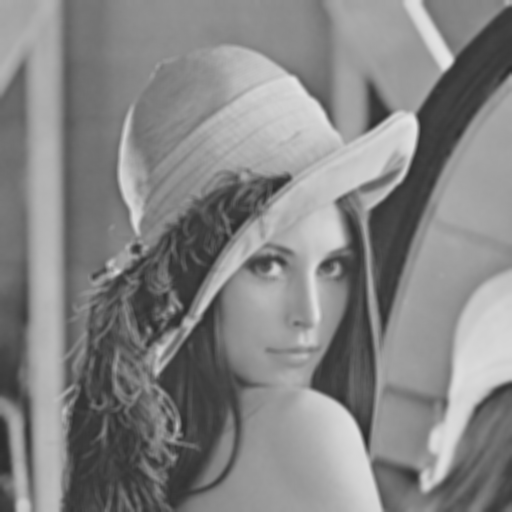
\includegraphics[scale=0.4]{imagenes/kernel.png}}
	\caption{Comparación de las imágenes\label{fig:kernel}.}
\end{figure}	

\begin{figure}[H]
	\centering
	\subfigure[Histograma de la imagen original]{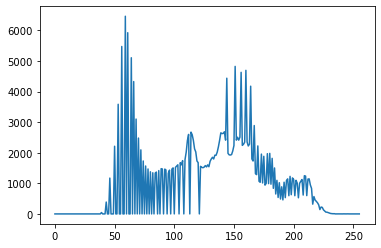
\includegraphics[scale=0.5]{imagenes/histOriginal.png}}
		\subfigure[Histograma de la imagen filtrada por \textit{Kernel}]{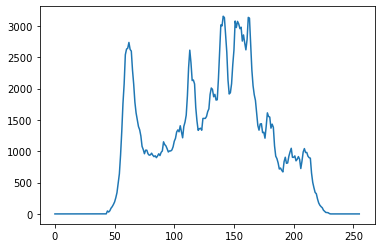
\includegraphics[scale=0.5]{imagenes/histKernel.png}}
	\caption{Comparación de los histogramas de las imágenes\label{fig:kernelhist}.}
\end{figure}	

\section{Banco de Filtro}

En la figura (\ref{fig:bf}), se observa el sistema tradicional del banco de filtro, en donde se aplica a una señal $x[n]$ se le aplica N filtros. Los filtros H sirve para quedarnos con los \textit{MxM} pixel de la imagen, por lo que termina siendo una matriz \textbf{H} igual

\begin{equation}
H=\begin{bmatrix}
1&\ldots&1\\
\vdots&\ddots&\vdots\\
1&\ldots&1\\
\end{bmatrix}
\end{equation}

de \textit{MxM}, y cada filtro se le aplica a una parte diferente de la imagen, esto seria parecido a un zoom aplicado anteriormente. Por ende, para realizar un zoom a una imagen con banco de filtro, consiste en ir aplicando banco de filtros consecutivos hasta obtener el zoom deseado ya que me va \textit{Downsapling} la señal filtrada. En una imagen, se tendría que la imagen original de \textit{512x512} se divide en 4 imágenes de \textit{256x256} (quedándome con el zoom de cada región) y luego se vuelve a dividir en 4 dando 8 imágenes de \textit{128x128} (banco de filtro consecutivo) y asi hasta obtener el zoom deseado. 

\begin{figure}[H]
	\centering
	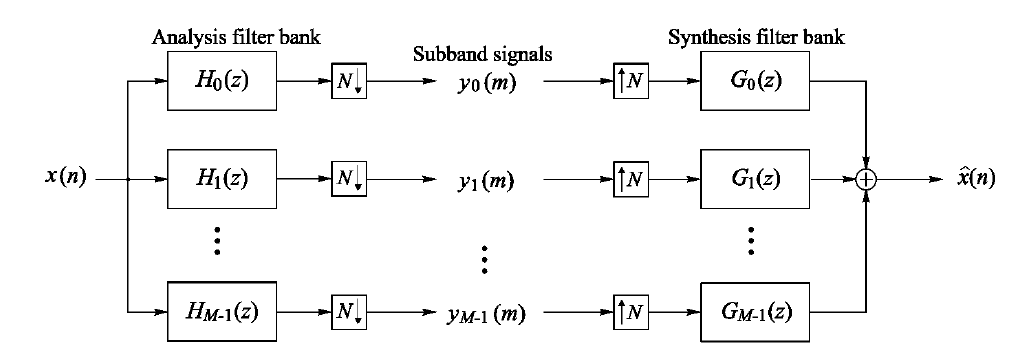
\includegraphics[scale=0.5]{imagenes/bancoFiltro.png}
	\caption{Sistema del banco de filtro\label{fig:bf}.}
\end{figure}

En este trabajo se realizo una división de sub bandas, tomadas de a 2 para mostrar la continuidad de aplicar banco de filtros. También, se uso un banco de filtro simple con $N=4$ y se le aplico a cada sub señal un filtro diferente para mostrar las aplicaciones de banco de filtro.

\subsubsection{Sub-Bandas}


	La figura (\ref{fig:sb}), muestra el sistema de sub bandas usando banco de filtro, en donde se observa que se va dividiendo la imagen en regiones de 2 hasta un limite $K$. La idea de realizar subbanding es mostrar el proceso que realiza bancos de filtros consecutivos. La imagen (\ref{fig:bf1}) muestra la imagen original mientras que (\ref{fig:bf2}) muestra la división hecha con los ancos de filtros consecutivos. Por ultimo, se tienen las imagenes (\ref{fig:bf3}) y  (\ref{fig:bf4}) correspode a la imagen aplicando el banco de filtro de la figura (\ref{fig:sb}) pero con una codificación de 0.2 bits por pixel  0.1 bits por pixel.
	
\begin{figure}[H]
	\centering
	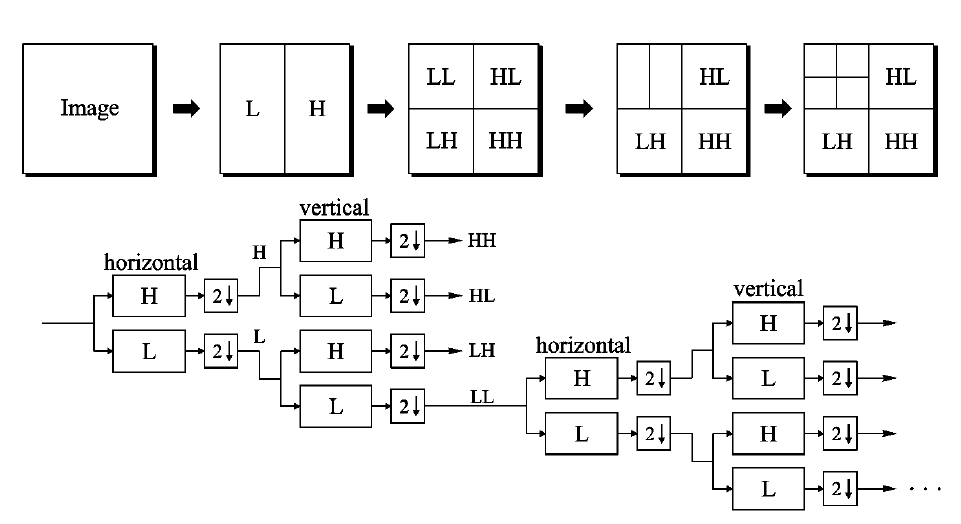
\includegraphics[scale=0.5]{imagenes/subBand.png}
	\caption{Sistema usado para la division de sub bandas.\label{fig:sb}.}
\end{figure}

\begin{figure}[H]
	\centering
	\subfigure[Imagen original \label{fig:bf1}]{\includegraphics[scale=0.5]{imagenes/subBand1.png}}
	\subfigure[Banco de filtro aplicado \label{fig:bf2}]{\includegraphics[scale=0.5]{imagenes/subBand2.png}}
	\subfigure[Codificacion de la imagen con 0.2 bits por pixel\label{fig:bf3}]{\includegraphics[scale=0.5]{imagenes/subBand3.png}}
	\subfigure[Codificacion de la imagen con 0.1 bits por pixel\label{fig:bf4}]{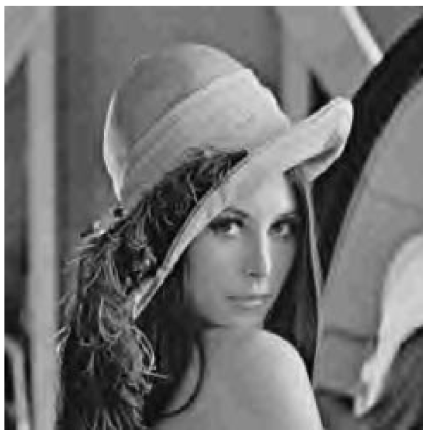
\includegraphics[scale=0.5]{imagenes/subBand4.png}}
	\caption{Comparación de las imágenes resultante\label{fig:sobel}.}
\end{figure}	

\section{Filtrado por partes con banco de filtro}

En esta sección, mostraremos el resultado de usar el banco de filtro en una aplicación concreta como en el filtrado de una imagen. Como vimos antes, un banco de filtro me permite trabajar con bandas de la señal de entrada permitiendo aplicar diferentes filtros en diferentes información de la señal de entrada. La figura (\ref{fig:bff}) realiza esto mismo, divido la imagen original en cuatro bandas permitiendo filtrar cada sub imagen con un filtro distinto de los mencionados anteriormente. En la figura, la parte superior izquierda corresponde al filtrado con el método \textit{Outline}, la parte superior derecha corresponde al método \textit{Sharpen}, la parte inferior izquierda corresponde al método \textit{Kernel} y la parte inferior derecha corresponde al método \textit{Right Sobel}.

\begin{figure}[H]
	\centering
	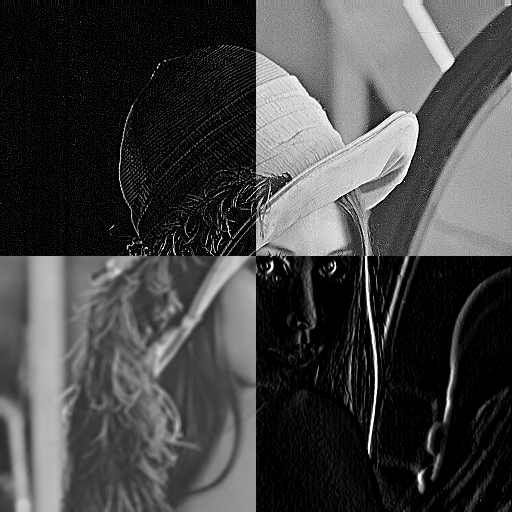
\includegraphics[scale=0.5]{imagenes/imgBf1.png}
	\caption{Imagen resultante de haber aplicado 4 filtro distintos con banco de filtros.\label{fig:bff}}
\end{figure}

\section{Conclusiones}


	Al realizar el trabajo se tubo que tener en cuenta tanta la imagen usada en formato con su respectivo header como los filtros a aplicar. Es importante destacar que cada filtro tiene su función particular para poder modificar la imagen permitiendo diferentes resultados.
	 
	Como se menciono es importante destacar los valores de la matrices \textbf{A} ya que si fueran cualquier otro numero podría dar un resultado totalmente diferente. 
	
	Por ultimo, mencionar la uso de los banco de filtros para realizar diferentes aplicaciones sobre la señal de entrada,tanto como estimar como para realizar operaciones sobre ellas (anular frecuencias, borrar datos de poco interés, etc) permitiendo trabajar sobre diferentes bandas de la señal.
